\scanpage{86}
% archive foliation: 85
$X$ schéma.

1.1. Données équivalentes

a) fibré en droites projectives \inserted{$P$} sur $X$
(fibré de Br. Sev. de rang 1)
\[
f:P\longrightarrow X
\]
b) ``\unsure{Module|fibré} loc. libre \inserted{rang 2, $E$}
mod \unsure{tensorisation|association} par
modules inversibles'' sur $X$

c) Algèbre d'Azumaya \inserted{$M$} de rang 4
\margin{si 2 inv. sur $X$}

\[
\left\{\begin{array}{ll}
\text{d)}&\text{Algèbre de Lie }\mathfrak g\quad
\text{forme }\inserted{\text{(type)}}\text{ de }\mathfrak{gp}(1)_X\\
\text{d')}&\rule{3cm}{.3pt}\ \mathfrak g'\ \rule{2cm}{.3pt}\quad
\deleted{\unsure{\mathfrak{gp}}}\mathfrak{sl}(\unsure{1|2})_X
\end{array}\right.
\]
e) forme $G$ de $\underline{GP}(1)_X$

\deleted{\unsure{e'}} \unsure{e')|e\textsuperscript{bis})}
\rule{1cm}{.3pt} $G'$ de $\underline{SL}(2)_X$

Si on a $P$, on en déduit
\[
E=f_*(L),\quad \underline L\text{ module inv. sur }P
\text{ de degré 1 sur \unsure{ch.que|ch. une} fibre}
\]
($\underline L$ défini loc. fppf \inserted{sur $X$} ou loc ét., mod
tensorisation par $f^*(\lambda)$, $\lambda$ inv. sur $X$)
\[
M=\check E\otimes E\simeq\underline{\operatorname{End}}(E)
\simeq E\otimes E\otimes(\Lambda^2E)^{-1}
\]
ext. de
\[
\underline O_X\ (\simeq\Lambda^2E\otimes(\Lambda^2E)^{-1})
\quad\text{par}\quad\Gamma^2E\otimes(\Lambda^2E)^{-1}
\]
ext. de
\[
\operatorname{Sym}^2(E)\otimes(\Lambda^2E)^{-1}
\quad\text{par}\quad\underline O_X\ (\simeq\Lambda^2E\otimes(\Lambda^2E)^{-1})
\]
\inserted{\[
f_*(L^{\otimes2})\otimes(\Lambda^2E)^{-1}
\simeq f_*(\underbrace{L^{\otimes2}\otimes\unsure{f^*\Lambda^2E|f^*(\Lambda^2E)^{-1}}}_{\underline t_{P/X}})
\]}

\margin{\unsure{expliciter|expliquer} !; ]
\diagram{\begin{tikzcd}[row sep=small]
\operatorname{Sym}^2E\otimes\operatorname{Sym}^2E\arrow[d]\\
\operatorname{Sym}^2E\otimes\Lambda^2E
\end{tikzcd}}
et
\diagram{\begin{tikzcd}[row sep=small]
\Gamma^2E\otimes\Gamma^2E\arrow[d]\\
\Gamma^2E\otimes\Lambda^2E
\end{tikzcd}}
\unsure{et accouplements|et couplages}
formes de Killing
\diagram{\begin{tikzcd}[column sep=small,row sep=small]
\operatorname{Sym}^2E\otimes\operatorname{Sym}^2E\arrow[r]
&(\Lambda^2E)^{\unsure{\otimes2}}\\
\Gamma^2E\otimes\Gamma^2E\arrow[ur]&
\end{tikzcd}}}
\figure{\begin{tikzpicture}[x=1cm,y=1cm]
\draw (0,4)--(1,4.1) to[bend left=30] (2,3.4)--(1.4,.5)--(0,0);
\end{tikzpicture}}

\[
M\overset{?}{\simeq}f_*\bigl(P^1_{P/X}(\underline t_{P/X})\bigr)
\quad\unsure{\text{additivement}|\text{ad libitum}}\ ?
\]
\[
\mathfrak g=M/\underline O_X
\]
avec crochet déduit du crochet \inserted{$(xy-yx)$}
de $M$ [\uline{NB} $\underline O_X$ en est le centre]
\[
\simeq f_*(\underline t_{P/X})
\]
[avec crochet provenant du crochet dans $\underline t_{P/X}$]

\[
\mathfrak g'\subset M^{\unsure{=\,\ell|\ell}}
\]
sous-algèbre des éléments de trace réduite nulle

($\mathfrak g'\longrightarrow\mathfrak g$ can, iso si 2 inv. sur $X$)
\[
\Vert\qquad\mathfrak g'\subset\check E\otimes E^{\unsure{\ell}}
\]
sous-algèbre des él. de trace nulle

\[
G=\operatorname{Aut}_X P,\qquad
G'=\widetilde G\quad\text{(rev. univ. de Chevalley)}
\]
\[
=\deleted{\operatorname{Aut}}\underline{SL}(E)
\]
\margin{\[
\begin{aligned}
G&\simeq\underline{\operatorname{Aut}}(E)/G_{mX}\\
&\simeq\underline{\operatorname{Aut}}(M)\\
&\simeq\underline{\operatorname{Aut}}(\mathfrak g)\\
&\simeq\underline{\operatorname{Aut}}(\mathfrak g')
\end{aligned}
\]
! attention à la Car. (notamment Car. 2!)}
\figure{\begin{tikzpicture}[x=1cm,y=1cm]
\draw (2,2)--(0,0)--(1.7,1.3);
\draw (2.5,2.7) to[bend right=20] (2.7,1.5)
to[bend left=40] (3,.9) to[bend left=40] (2.7,.5)
to[bend right=20] (2.5,-.5);
\end{tikzpicture}}

$P=\mathbb P(E)=$ schéma des Idéaux à gauche
qui sont ``spéciaux'' i.e. loc. fact. directs et
``non \uline{\unsure{triviaux en aucun point|triviaux}}''
\deleted{\unsure{sur $X$}}

$=$ schéma des sous-Alg. de Borel de $\mathfrak g$
\figure{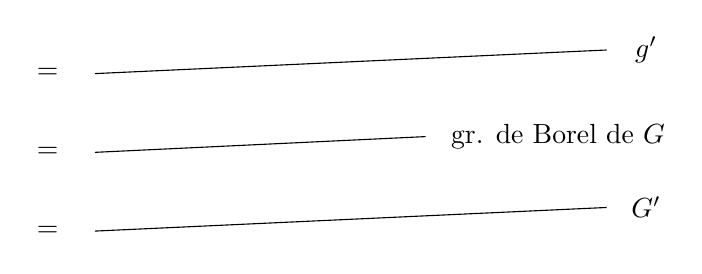
\begin{tikzpicture}[x=1cm,y=1cm]
\node at (0,2) {$=$};\draw (.6,2)--(7.1,2.3);\node at (7.6,2.3) {$\mathfrak g'$};
\node at (0,1) {$=$};\draw (.6,1)--(4.8,1.2);
\node[anchor=west] at (5,1.2) {gr. de Borel de $G$};
\node at (0,0) {$=$};\draw (.6,0)--(7.1,.3);\node at (7.6,.3) {$G'$};
\end{tikzpicture}}

